\setbeamercovered{transparent}
\begin{frame}{Объектно-центричное обучение}
    \begin{itemize}
        \item<1-4> Базовое предположение: наблюдение состоит из $N$ объектов, каждый из которых может быть смоделирован по отдельности
        \item<2-4> Объекты могут взаимодействовать друг с другом и влиять друг на друга
        \item<3-4> Объектная абстракция позволяет ввести структуру в наблюдения, представленные изображениями в таких задачах, как предсказание видео или визуальный контроль в обучении с подкреплением
        \item<4> Может быть применено для повышения скорости обучения и обобщающих способностей в обучении с подкреплением
    \end{itemize}
    
\end{frame}
\setbeamercovered{invisible}

% \begin{frame}{Object-Centric Learning with Slot Attention \cite{SlotAttention}, NIPS'20 }
%     \begin{columns}
%     \begin{column}{0.7\textwidth}
%     \begin{itemize}
%         \item Object-centric approach to representation learning
%         \item Main contribution - Slot Attention module
%         \item Maps $N$ input feature vectors to $K$ \textit{slots}
%     \end{itemize}
%     \end{column}
%     \begin{column}{0.4\textwidth}
%     \begin{figure}
%         \centering
%         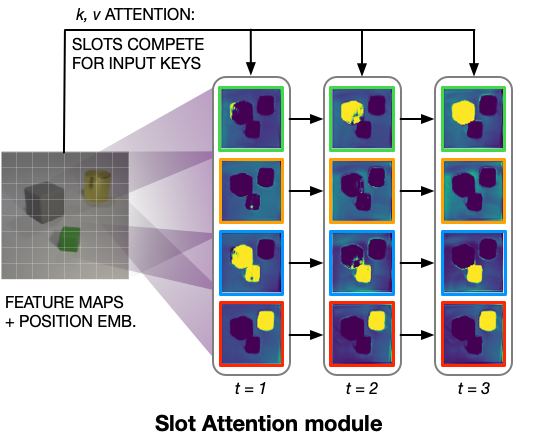
\includegraphics[width=\linewidth]{images/rel_work/slot_att_scheme.png}
%         % \caption{Slot Attention Scheme}
%         % \label{fig:slot_att}
%     \end{figure}
%     \end{column}
%     \end{columns}
% \end{frame}

% \begin{frame}{Object-Centric Learning with Slot Attention \cite{SlotAttention}, NIPS'20}
%     \begin{columns}
%     \begin{column}{0.45\textwidth}
%     Applications:
%     \begin{itemize}
%         \item Unsupervised object discovery
%         \begin{itemize}
%             \item Number of slots is hyperparameter
%         \end{itemize}
%         \item Set prediction
%         \begin{itemize}
%             \item Sets are predicted with MLP
%         \end{itemize}
%     \end{itemize}
%     \begin{figure}
%         \centering
%         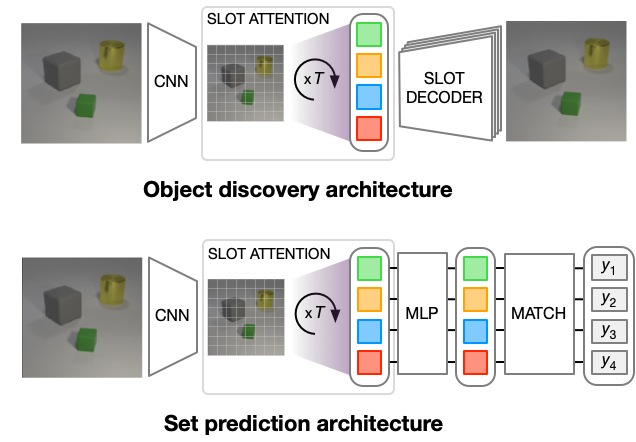
\includegraphics[width=\linewidth]{images/rel_work/slot_att_arch.png}
%         % \caption{Object detection experiment}
%         % \label{fig:slot_att_obj_detect}
%     \end{figure}
%     \end{column}
    
%     \begin{column}{0.45\textwidth}
%     \begin{figure}
%         \centering
%         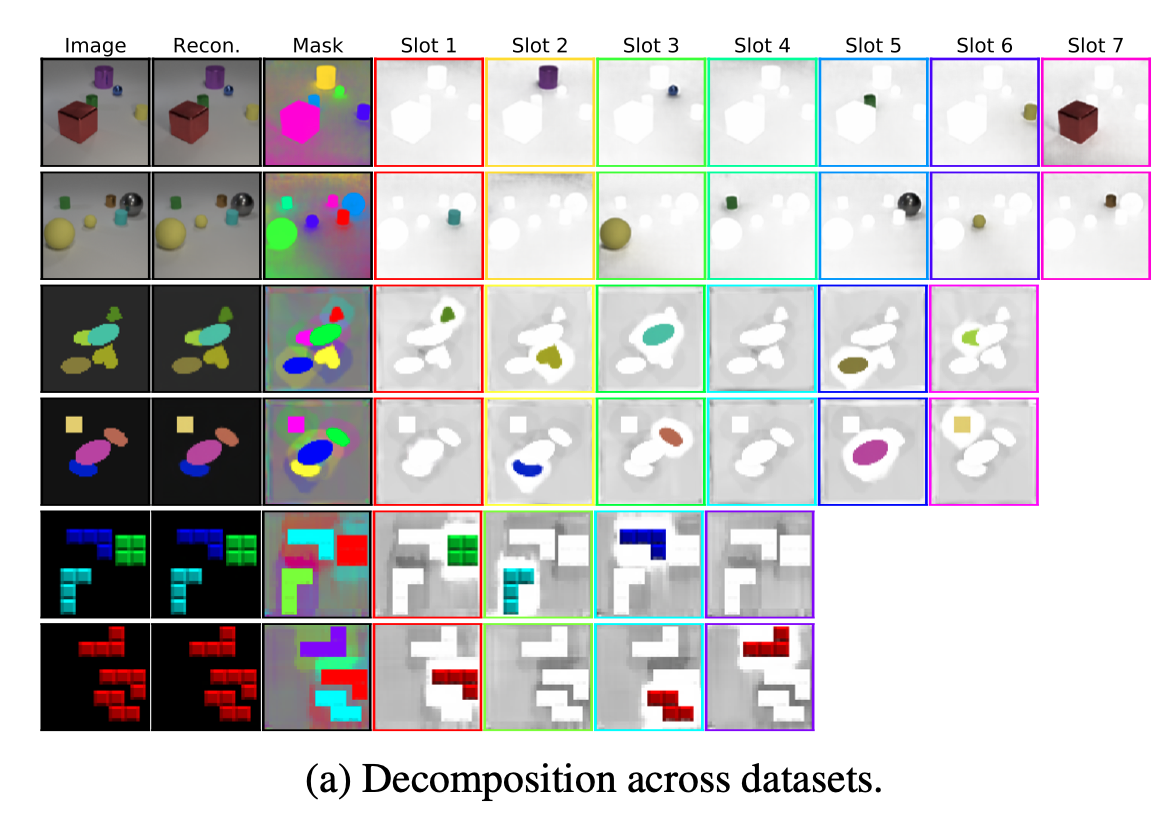
\includegraphics[width=\linewidth]{images/rel_work/slot_att_obj_recogn.png}
%         % \caption{Object detection experiment}
%         % \label{fig:slot_att_obj_detect}
%     \end{figure}
%     \end{column}
%     \end{columns}
% \end{frame}

% \begin{frame}{Contrastive Learning of Structured World Models \cite{cSWM}, ICLR'20}
%     \begin{itemize}
%         \item Both action and state spaces are factorized
%         \item Transition model is message-passing GNN
%         \item Multi-object contrastive learning using samples from buffer
%     \end{itemize}
%     \begin{figure}
%         \centering
%         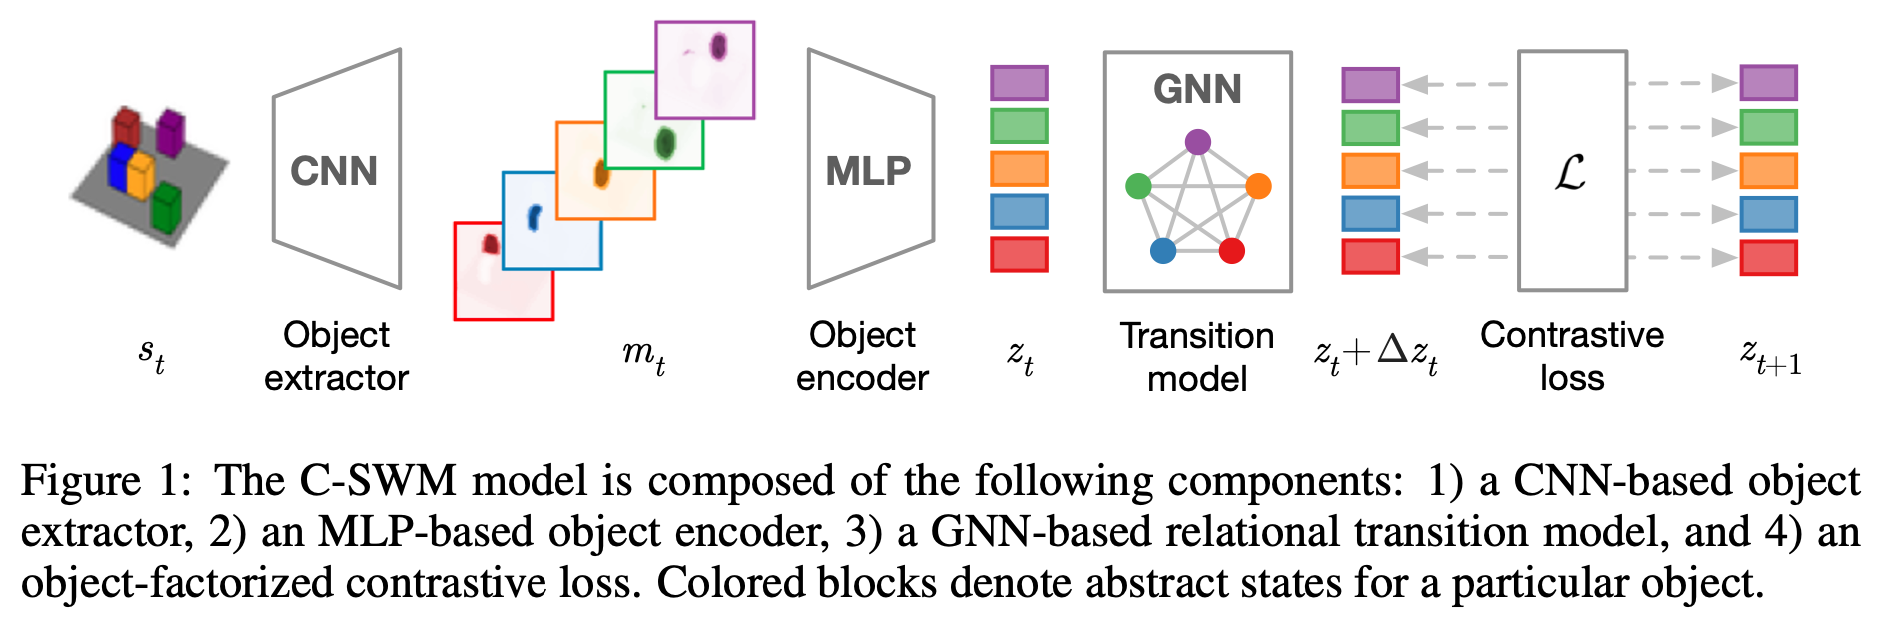
\includegraphics[height=0.3\paperheight]{images/rel_work/cswm_scheme.png}
%         % \caption{C-SWM scheme}
%         % \label{fig:cswm_scheme}
%     \end{figure}
% \end{frame}
% \begin{frame}{Contrastive Learning of Structured World Models \cite{cSWM}, ICLR'20}
%     Experiments:
%     \begin{itemize}
%         \item Multiple environments with different moving objects
%         \item Atari Pong and Space Invaders
%         \item Objective - predict the next observation after taking the action/actions.
%     \end{itemize}
%     \begin{figure}
%         \centering
%         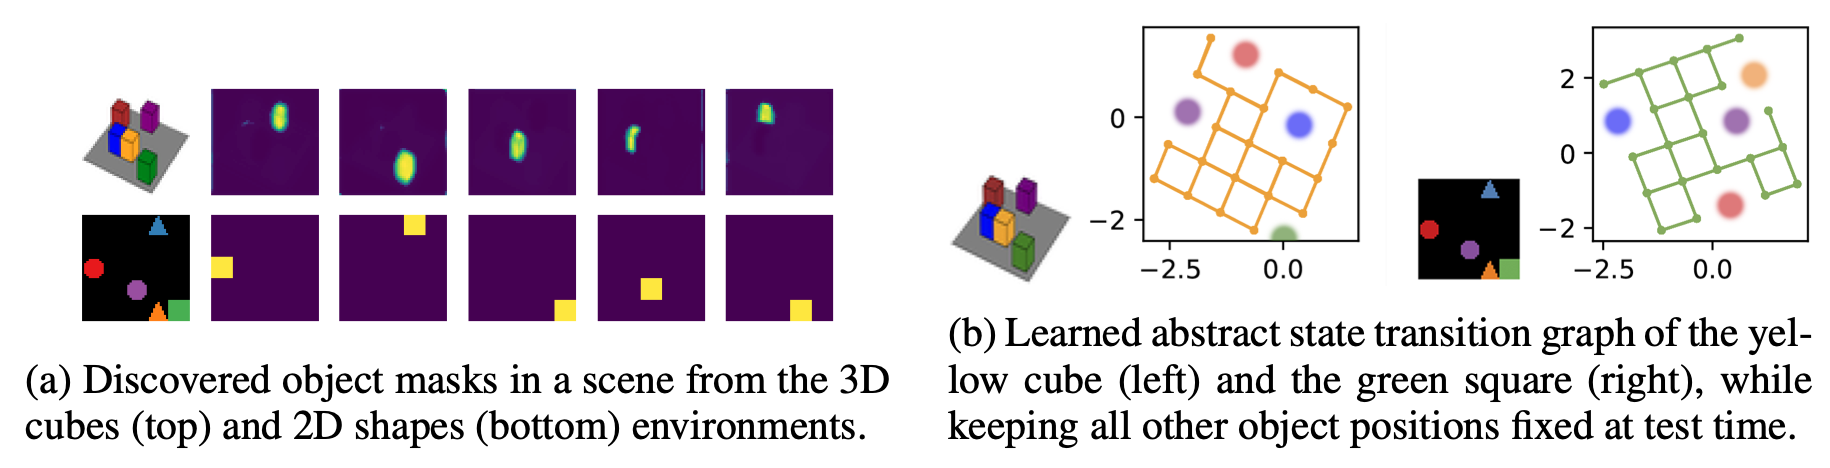
\includegraphics[height=0.3\paperheight]{images/rel_work/cswm_predictions.png}
%         % \caption{CSWM experiment results}
%         % \label{fig:my_label}
%     \end{figure}
% \end{frame}

% \begin{frame}{Entity Abstraction in Visual Model-Based Reinforcement Learning \cite{OP3}, CoRL'19}
%     \begin{itemize}
%         \item Generalization via modeling universal interaction and entities
%         \item Designed for combinatorical tasks with similar objects
%         \item Can be applied for goal-conditioned RL and object detection in videos
%     \end{itemize}
%     \begin{figure}
%         \centering
%         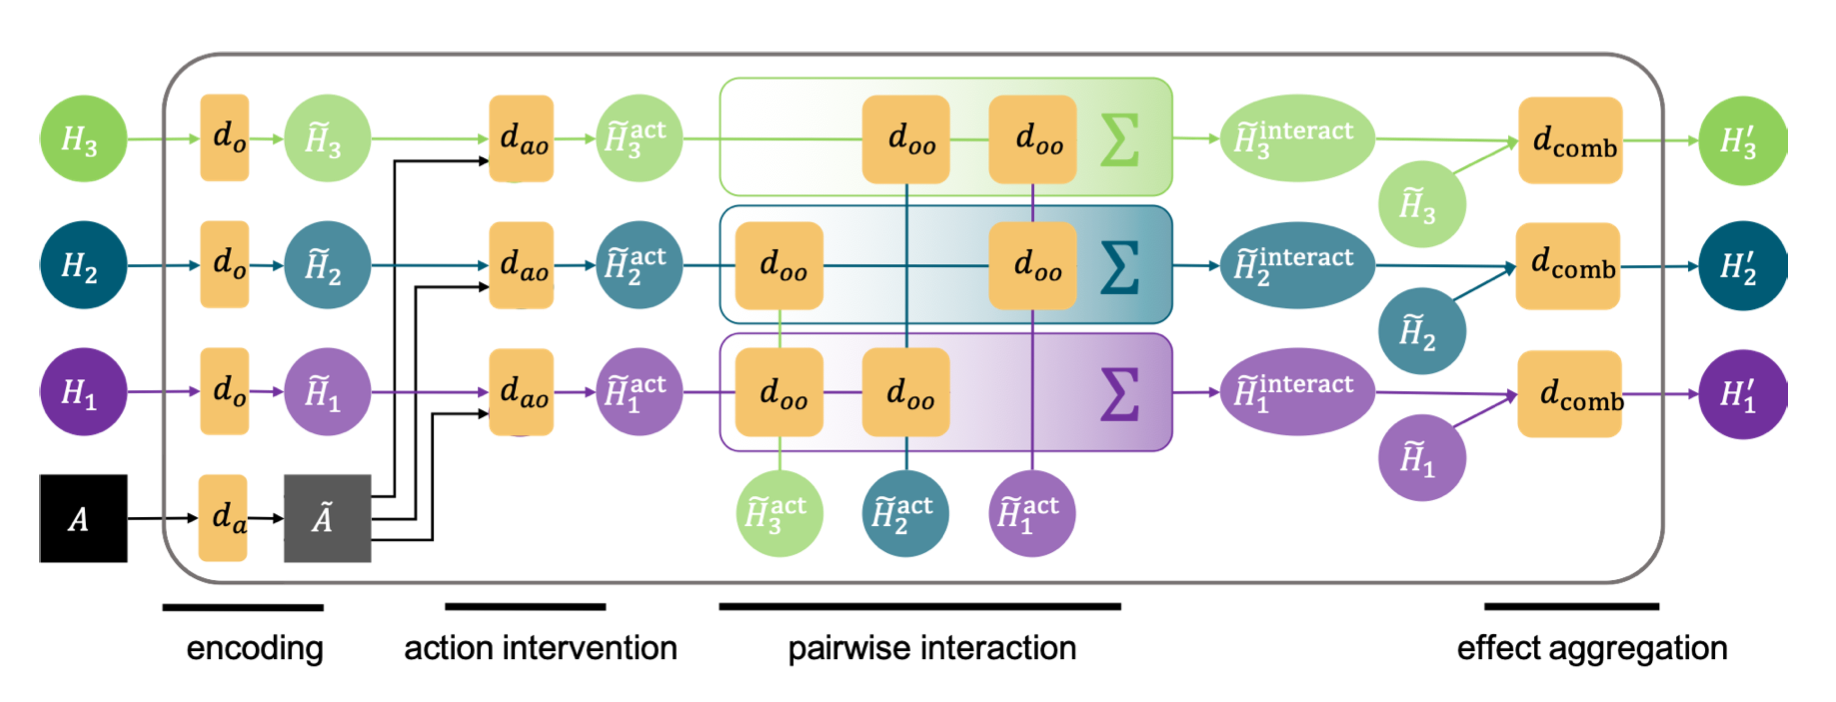
\includegraphics[height=0.3\paperheight]{images/rel_work/op3_dynamics.png}
%         % \caption{ROLL scheme}
%         % \label{fig:roll_scheme}
%     \end{figure}
% \end{frame}

% \begin{frame}{GATSBI: Generative Agent-centric Spatio-temporal Object Interaction \cite{GATSBI}, CVPR'21}
% \begin{columns}
% \begin{column}{0.45\textwidth}
%     \begin{itemize}
%         \item Unsupervised spatio-temporal representation
%         \item Three entity categories
%         \item GMM for grounding large components
%         \item Keypoint module for robot, attention-based object module
%         \item Interactions as GNN consider different nature of objects
%     \end{itemize}
% \end{column}
% \begin{column}{0.45\textwidth}
%     \begin{figure}
%         \centering
%         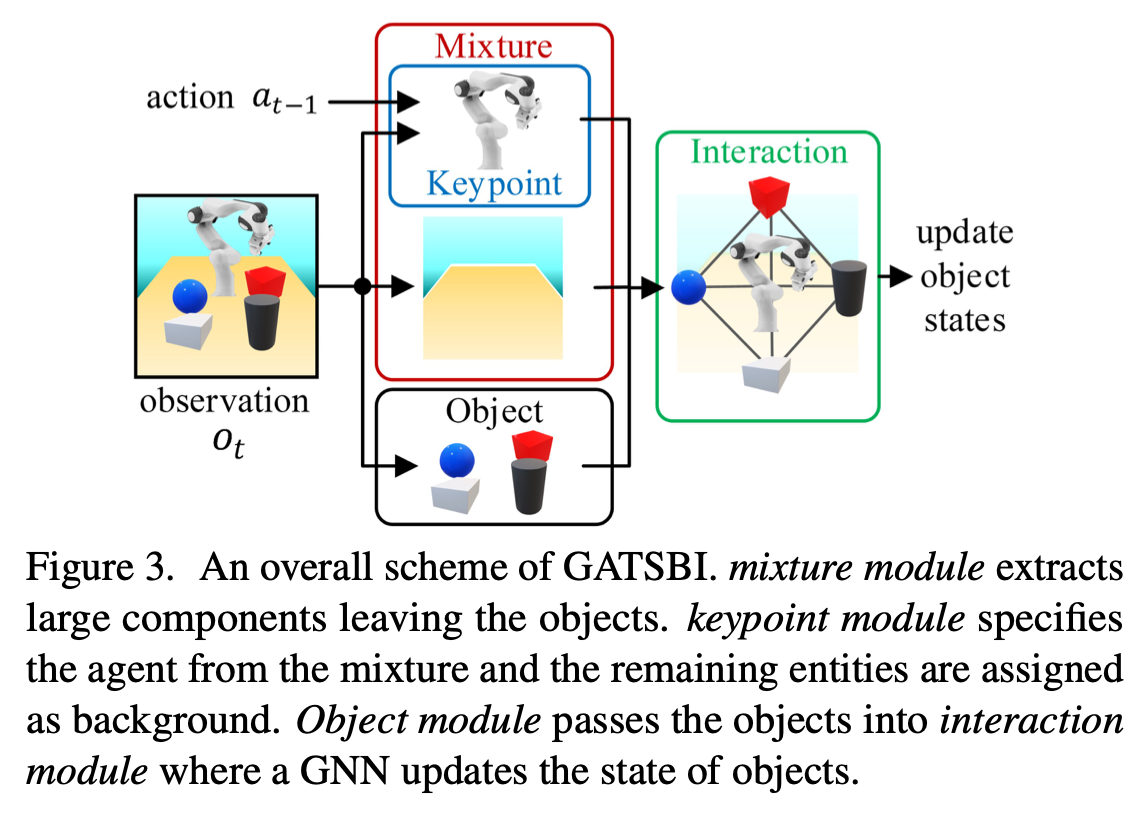
\includegraphics[width=\linewidth]{images/rel_work/gatsbi_scheme.png}
%         % \caption{ROLL scheme}
%         % \label{fig:roll_scheme}
%     \end{figure}
% \end{column}
% \end{columns}
% \end{frame}

% \begin{frame}{ROLL: Visual Self-Supervised Reinforcement Learning with Object Reasoning \cite{ROLL}, CoRL'20}
% \begin{columns}
% \begin{column}{0.45\textwidth}
%     \begin{itemize}
%         \item Object-centric approach to goal-conditioned RL
%         \item Explicitly segmented robot, background and objects
%         \item Deals with occluded objects
%     \end{itemize}
% \end{column}
% \begin{column}{0.45\textwidth}
%     \begin{itemize}
%         \item Works under assumptions that background is static and reward depends on the object position
%         \item Most of the training performed offline
%     \end{itemize}
% \end{column}
% \end{columns}
% \begin{figure}
%     \centering
%     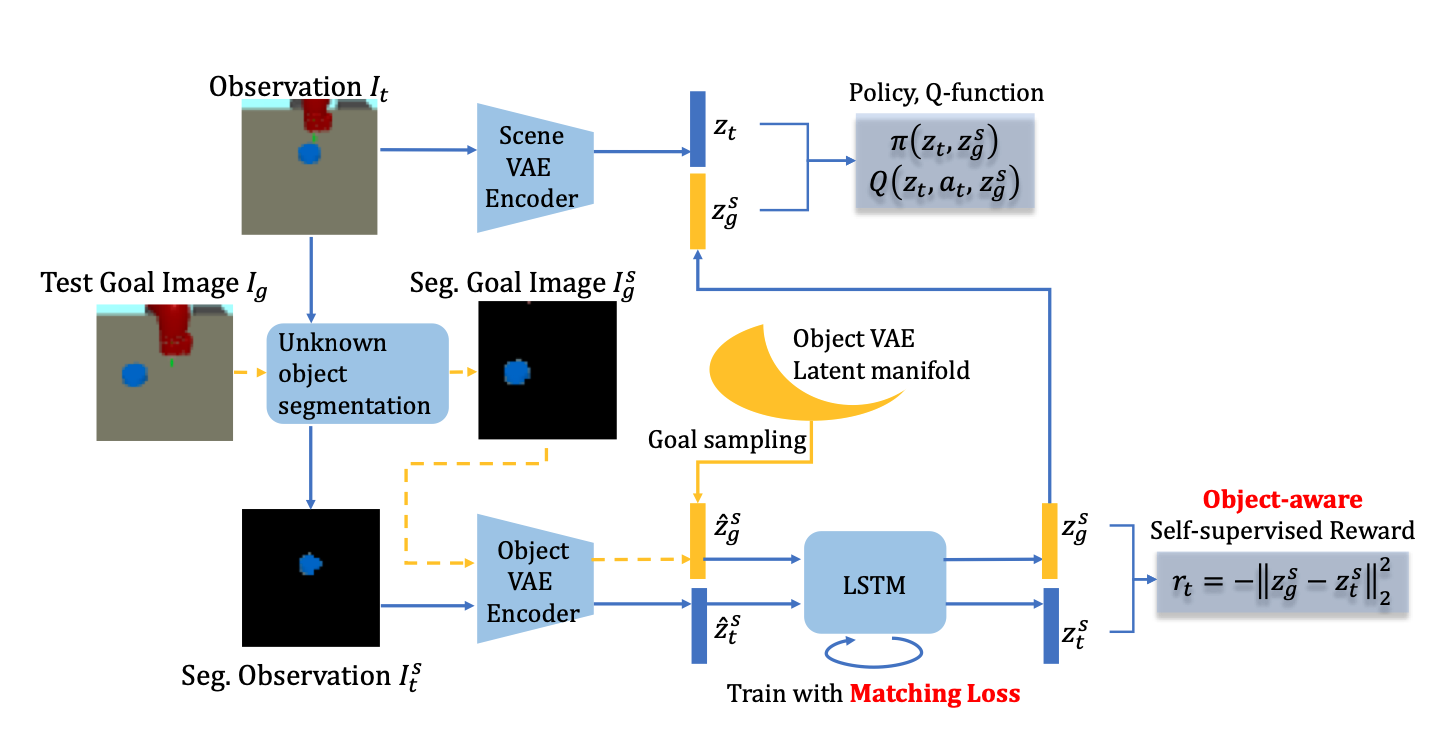
\includegraphics[height=0.4\paperheight]{images/rel_work/roll_scheme.png}
%     % \caption{ROLL scheme}
%     % \label{fig:roll_scheme}
% \end{figure}
% \end{frame}

% \begin{frame}{CAI \cite{CAI}, NIPS'21}
%     \begin{itemize}
%         \item Causal Influence Detection for Improving Efficiency in RL
%         \item Interactions as causal graph
%         \item Control is quantified and measured
%         \item Applications to RL:
%         \begin{itemize}
%             \item Reward bonus for Causal Action Influence (CAI)
%             \item Exploratory policy using CAI
%             \item Causal Influence-based Experience Replay
%         \end{itemize}
%     \end{itemize}
%     \begin{figure}
%         \centering
%         \includegraphics[height=0.3\paperheight]{images/rel_work/causal_scheme.png}
%         % \caption{ROLL scheme}
%         % \label{fig:roll_scheme}
%     \end{figure}
% \end{frame}